\documentclass[11pt]{article}
\makeatletter\if@twocolumn\PassOptionsToPackage{switch}{lineno}\else\fi\makeatother

      \makeatletter
\usepackage{wrapfig}
\newcounter{aubio}

\long\def\bioItem{%
\@ifnextchar[{\@bioItem}{\@@bioItem}}

\long\def\@bioItem[#1]#2#3{
 \stepcounter{aubio}
 \expandafter\gdef\csname authorImage\theaubio\endcsname{#1}
 \expandafter\gdef\csname authorName\theaubio\endcsname{#2}
 \expandafter\gdef\csname authorDetails\theaubio\endcsname{#3}
}

\long\def\@@bioItem#1#2{
 \stepcounter{aubio}
 \expandafter\gdef\csname authorName\theaubio\endcsname{#1}
 \expandafter\gdef\csname authorDetails\theaubio\endcsname{#2}
}

\newcommand{\checkheight}[1]{%
  \par \penalty-100\begingroup%
  \setbox8=\hbox{#1}%
  \setlength{\dimen@}{\ht8}%
  \dimen@ii\pagegoal \advance\dimen@ii-\pagetotal
  \ifdim \dimen@>\dimen@ii
    \break
  \fi\endgroup}

\def\printBio{%
  \@tempcnta=0
   \loop
     \advance \@tempcnta by 1
     \def\aubioCnt{\the\@tempcnta}
     \setlength{\intextsep}{0pt}%
     \setlength{\columnsep}{10pt}%
     \newbox\boxa%
     \setbox\boxa\vbox{\csname authorDetails\aubioCnt\endcsname}
     \expandafter\ifx\csname authorImage\aubioCnt\endcsname\relax%
      \else%
       \checkheight{\includegraphics[height=1.25in,width=1in,keepaspectratio]{\csname authorImage\aubioCnt\endcsname}}
        \begin{wrapfigure}{l}{25mm}
         \includegraphics[height=1.25in,width=1in,keepaspectratio]{\csname authorImage\aubioCnt\endcsname}%height=145pt
        \end{wrapfigure}\par
      \fi
     {\parindent0pt\textbf{\csname authorName\aubioCnt\endcsname}\csname authorDetails\aubioCnt\endcsname \par\bigskip%
     \expandafter\ifx\csname authorImage\aubioCnt\endcsname\relax\else%
      \ifdim\the\ht\boxa < 90pt\vskip\dimexpr(90pt -\the\ht\boxa-1pc)\fi%
     \fi}%for adding additional vskip for avoiding image overlap.
      \ifnum\@tempcnta < \theaubio
   \repeat
   }

\makeatother

      



\usepackage{amsfonts,amssymb,amsbsy,latexsym,amsmath,tabulary,graphicx,times,xcolor}
\usepackage[utf8x]{inputenc}
\usepackage{fancyhdr}
\def\NormalBaseline{\def\baselinestretch{1.1}}
\makeatletter
\def\hlinewd#1{%
  \noalign{\ifnum0=`}\fi\hrule \@height #1%
  \futurelet\reserved@a\@xhline}
\def\tbltoprule{\hlinewd{.8pt}}%\\[-10pt]}
\def\tblbottomrule{\hlinewd{.8pt}}
\def\tblmidrule{\hline\noalign{\vspace*{2pt}}}

\def\@shorttitle{\@empty}
\def\shorttitle#1{\gdef\@shorttitle{#1}}

\fancypagestyle{custom}{
\fancyhf{}
\fancyhead[C]{\@shorttitle}
\fancyhead[R]{\thepage}
\fancyfoot[C]{}
\renewcommand\headrulewidth{0.4pt}
\renewcommand\footrulewidth{0pt}
}
\fancypagestyle{plain}{
\fancyhf{}
\renewcommand\headrulewidth{0.4pt}
}


\makeatother

\usepackage{times}

\usepackage[a4paper,margin=2.5cm,headsep=.7cm,headheight=18pt,top=3cm,footnotesep=1.5\baselineskip]{geometry}
\usepackage{caption}
\captionsetup[figure]{labelfont=bf,labelsep=newline,justification=centerlast,labelfont={small,sc,bf},font=small,aboveskip=.3\baselineskip}

\captionsetup[table]{labelfont=bf,labelsep=newline,justification=centerlast,labelfont={small,sc,bf},font=small,aboveskip=.3\baselineskip}
\linespread{1.5}

\setcounter{totalnumber}{4}
\def\topfraction{0.9}
\def\bottomfraction{0.4}
\def\floatpagefraction{0.8}
\def\textfraction{0.1}
\widowpenalty 10000
\clubpenalty 10000
\makeatletter
\setlength\intextsep   {1.5\baselineskip \@plus 2\p@ \@minus 2\p@}
\makeatother

  
%%%%%%%%%%%%%%%%%%%%%%%%%%%%%%%%%%%%%%%%%%%%%%%%%%%%%%%%%%%%%%%%%%%%%%%%%%
% Following additional macros are required to function some 
% functions which are not available in the class used.
%%%%%%%%%%%%%%%%%%%%%%%%%%%%%%%%%%%%%%%%%%%%%%%%%%%%%%%%%%%%%%%%%%%%%%%%%%
\usepackage{url,multirow,morefloats,floatflt,cancel,tfrupee}
\makeatletter


\AtBeginDocument{\@ifpackageloaded{textcomp}{}{\usepackage{textcomp}}}
\makeatother
\usepackage{colortbl}
\usepackage{xcolor}
\usepackage{pifont}
\usepackage[nointegrals]{wasysym}
\urlstyle{rm}
\makeatletter

%%%For Table column width calculation.
\def\mcWidth#1{\csname TY@F#1\endcsname+\tabcolsep}

%%Hacking center and right align for table
\def\cAlignHack{\rightskip\@flushglue\leftskip\@flushglue\parindent\z@\parfillskip\z@skip}
\def\rAlignHack{\rightskip\z@skip\leftskip\@flushglue \parindent\z@\parfillskip\z@skip}

%Etal definition in references
\@ifundefined{etal}{\def\etal{\textit{et~al}}}{}


%\if@twocolumn\usepackage{dblfloatfix}\fi
\usepackage{ifxetex}
\ifxetex\else\if@twocolumn\@ifpackageloaded{stfloats}{}{\usepackage{dblfloatfix}}\fi\fi

\AtBeginDocument{
\expandafter\ifx\csname eqalign\endcsname\relax
\def\eqalign#1{\null\vcenter{\def\\{\cr}\openup\jot\m@th
  \ialign{\strut$\displaystyle{##}$\hfil&$\displaystyle{{}##}$\hfil
      \crcr#1\crcr}}\,}
\fi
}

%For fixing hardfail when unicode letters appear inside table with endfloat
\AtBeginDocument{%
  \@ifpackageloaded{endfloat}%
   {\renewcommand\efloat@iwrite[1]{\immediate\expandafter\protected@write\csname efloat@post#1\endcsname{}}}{\newif\ifefloat@tables}%
}%

\def\BreakURLText#1{\@tfor\brk@tempa:=#1\do{\brk@tempa\hskip0pt}}
\let\lt=<
\let\gt=>
\def\processVert{\ifmmode|\else\textbar\fi}
\let\processvert\processVert

\@ifundefined{subparagraph}{
\def\subparagraph{\@startsection{paragraph}{5}{2\parindent}{0ex plus 0.1ex minus 0.1ex}%
{0ex}{\normalfont\small\itshape}}%
}{}

% These are now gobbled, so won't appear in the PDF.
\newcommand\role[1]{\unskip}
\newcommand\aucollab[1]{\unskip}
  
\@ifundefined{tsGraphicsScaleX}{\gdef\tsGraphicsScaleX{1}}{}
\@ifundefined{tsGraphicsScaleY}{\gdef\tsGraphicsScaleY{.9}}{}
% To automatically resize figures to fit inside the text area
\def\checkGraphicsWidth{\ifdim\Gin@nat@width>\linewidth
	\tsGraphicsScaleX\linewidth\else\Gin@nat@width\fi}

\def\checkGraphicsHeight{\ifdim\Gin@nat@height>.9\textheight
	\tsGraphicsScaleY\textheight\else\Gin@nat@height\fi}

\def\fixFloatSize#1{}%\@ifundefined{processdelayedfloats}{\setbox0=\hbox{\includegraphics{#1}}\ifnum\wd0<\columnwidth\relax\renewenvironment{figure*}{\begin{figure}}{\end{figure}}\fi}{}}
\let\ts@includegraphics\includegraphics

\def\inlinegraphic[#1]#2{{\edef\@tempa{#1}\edef\baseline@shift{\ifx\@tempa\@empty0\else#1\fi}\edef\tempZ{\the\numexpr(\numexpr(\baseline@shift*\f@size/100))}\protect\raisebox{\tempZ pt}{\ts@includegraphics{#2}}}}

%\renewcommand{\includegraphics}[1]{\ts@includegraphics[width=\checkGraphicsWidth]{#1}}
\AtBeginDocument{\def\includegraphics{\@ifnextchar[{\ts@includegraphics}{\ts@includegraphics[width=\checkGraphicsWidth,height=\checkGraphicsHeight,keepaspectratio]}}}

\DeclareMathAlphabet{\mathpzc}{OT1}{pzc}{m}{it}

\def\URL#1#2{\@ifundefined{href}{#2}{\href{#1}{#2}}}

%%For url break
\def\UrlOrds{\do\*\do\-\do\~\do\'\do\"\do\-}%
\g@addto@macro{\UrlBreaks}{\UrlOrds}



\edef\fntEncoding{\f@encoding}
\def\EUoneEnc{EU1}
\makeatother
\def\floatpagefraction{0.8} 
\def\dblfloatpagefraction{0.8}
\def\style#1#2{#2}
\def\xxxguillemotleft{\fontencoding{T1}\selectfont\guillemotleft}
\def\xxxguillemotright{\fontencoding{T1}\selectfont\guillemotright}

\newif\ifmultipleabstract\multipleabstractfalse%
\newenvironment{typesetAbstractGroup}{}{}%

%%%%%%%%%%%%%%%%%%%%%%%%%%%%%%%%%%%%%%%%%%%%%%%%%%%%%%%%%%%%%%%%%%%%%%%%%%

\usepackage{natbib}




\usepackage{titlesec}
\usepackage[T1]{fontenc}
\setcounter{secnumdepth}{5}
 
\titleformat{\section}[hang]{\NormalBaseline\filright\large\bfseries}
{\large\thesection}
{10pt}
{}
[]
\titleformat{\subsection}[hang]{\NormalBaseline\filright\bfseries}
{\thesubsection}
{10pt}
{}
[]
\titleformat{\subsubsection}[hang]{\NormalBaseline\filright\bfseries\itshape}
{\upshape\thesubsubsection}
{10pt}
{}
[]
\titleformat{\paragraph}[runin]{\NormalBaseline\filright\bfseries}
{\theparagraph}
{10pt}
{}
[]
\titleformat{\subparagraph}[runin]{\NormalBaseline\filright\bfseries\itshape}
{\thesubparagraph}
{10pt}
{}
[]

\titlespacing{\section}{0pt}{1.5\baselineskip}{.2\baselineskip}  
\titlespacing{\subsection}{0pt}{1.5\baselineskip}{.2\baselineskip}  
\titlespacing{\subsubsection}{0pt}{1.5\baselineskip}{.2\baselineskip}  
\titlespacing{\paragraph}{0pt}{.5\baselineskip}{10pt}  
\titlespacing{\subparagraph}{0pt}{.5\baselineskip}{10pt}  
  

  




%%%%%%%%%%%%%%%%%%%%%%%%%%%%%%%%%%%%%%%%%%
% Feature enabled:
%secnum: unnumbered
%linespacing: 1.25
%%%%%%%%%%%%%%%%%%%%%%%%%%%%%%%%%%%%%%%%%%

\setcounter{secnumdepth}{0}

\linespread{1.25}

\usepackage{float}

\begin{document}



\renewcommand*\rmdefault{bch}\normalfont\upshape

\shorttitle{Sol-Gel Method}

\date{}  

  
\title{\NormalBaseline\raggedright\bfseries Homework 4a {\textemdash} Paper Review}
  \let\origthanks\thanks
\renewcommand\thanks[1]{\begingroup\let\rlap\relax\origthanks{#1}\endgroup}
\author{\hskip2pc\parbox{.95\textwidth}{\bfseries\large Antonio Osamu Katagiri Tanaka\textsuperscript{1}\thanks{E-mail: A01212611@itesm.mx}
      \\[3pt] 
    % Address
    \normalfont\itshape\NormalBaseline \textsuperscript{\upshape 1} 
    ITESM\unskip, \normalfont\itshape\NormalBaseline Av. Eugenio Garza Sada 2501 Sur\unskip, N.L.\unskip, Monterrey\unskip, Mexico}}
    
    
\maketitle 
\pagestyle{custom}

    
\section{Transformation of a Simple Plastic into a Superhydrophobic Surface\unskip~\protect\cite{691550:16648156}.}
Sol-gel method, introduced by Buckley and Greenblatt\unskip~\cite{691550:16609761}, is one of the well-established techniques to fabricate nano particles and structures. The processes involved in the sol-gel method are: hydrolysis, condensation, and drying. First the precursor in question undergoes rapid hydrolysis, followed by immediate condensation which leads to the formation of a gel. Finally, the obtained gel is subjected to drying process, to convert the generated gel into a xerogel or aerogel depending on the drying technique as shown in Figure~\ref{f-3fd2f63bd067}. 


\bgroup
\fixFloatSize{images/97ffa8fc-85fa-4186-9db1-199311d5f0ac-usolgelmethod.jpg}
\begin{figure*}[!htbp]
\centering \makeatletter\IfFileExists{images/97ffa8fc-85fa-4186-9db1-199311d5f0ac-usolgelmethod.jpg}{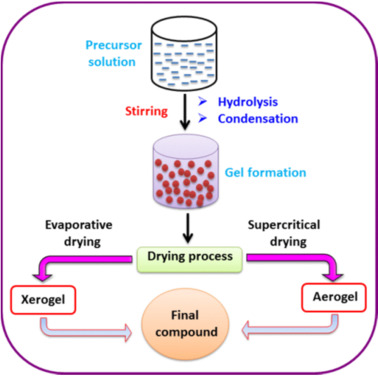
\includegraphics{images/97ffa8fc-85fa-4186-9db1-199311d5f0ac-usolgelmethod.jpg}}{}
\makeatother 
\caption{{The Sol{\textendash}Gel Method process\unskip~\protect\cite{691550:16646163}}}
\label{f-3fd2f63bd067}
\end{figure*}
\egroup
Erbil et al.\unskip~\cite{691550:16648156} implemented a variation of the Sol-gel method, in which they patterned the resulting get into a thin film before the drying process to create a superhydrophobic coating. Erbil et al. work intended to investigate the effect of polymer concentration, film formation temperature, and the non-solvent effects on the homogeneity, surface roughness, and water contact angle of isotactic polypropylene coatings. The authors' key takeaways are listed below.

\begin{itemize}
  \item \relax The hydrophobic property of a surface increases with the decrease of surface energy or by increasing the surface roughness.
  \item \relax The water contact angle increases with the increase of surface roughness, due to the roughness factor and the air pockets within the $\mu $ pores.
  \item \relax The coating thickness increases with increasing polymer concentration and surface roughness
  \item \relax Low drying temperatures result in an increase of homogeneous pores, and surface roughness, as the solvent evaporation rate is slower and the crystallization time is increased.
  \item \relax Non-solvents favor the polymer phase separation between two phases, increase the rate of evaporation, and aid the formation of homogeneous coatings.
\end{itemize}
  
    
\section{Alternate/Proposed method to create superhydrophobic surfaces.}
Erbil et al.'s approach could be amended. Instead of just dropping a few drops of the polymer solution onto the glass substrate, the polymer precursor could be deposited by some dip, spin or spray coating technique. On the other hand, lithography techniques could be implemented to simulate the surface roughness and hydrophobic properties with posts and walls. Furthermore, etching technique may also work to create hydrophobic surfaces. Instead of adding a coating, the existing surface could be modified to increase its roughness.

\clearpage 
    

\bibliographystyle{blank}

\bibliography{\jobname}

\section*{Author biography}

\bioItem[images/bf0f1284-fa36-4678-a9e7-05671376e50c-umeitesm]{Antonio Osamu Katagiri Tanaka}{ .

MNT16

A01212611}
\printBio 

\end{document}
